\documentclass[a4paper, 11pt]{article}
\usepackage[listings]{mypackage}
\usepackage{float}
\usepackage{amsmath}
\usepackage{graphicx}
\usepackage{geometry}
\usepackage{listings}
\usepackage[colorlinks,linkcolor=red]{hyperref}
\geometry{scale=0.8}

\title{	
\normalfont \normalsize
\textsc{School of Data and Computer Science, Sun Yat-sen University} \\ [25pt] %textsc small capital letters
\rule{\textwidth}{0.5pt} \\[0.4cm] % Thin top horizontal rule
\huge  Maze Problem (Lab 1)\\ % The assignment title
\rule{\textwidth}{2pt} \\[0.5cm] % Thick bottom horizontal rule
\author{17341015 Hongzheng Chen}
\date{\normalsize\today}
}

\lstset{language=Python}

\begin{document}
\maketitle
\tableofcontents
\newpage
\section{Task}

\begin{itemize}
	\item Please solve the maze problem (i.e., find the shortest path from the start point to the finish point) by using BFS or DFS (Python or C++)
	\item The maze layout can be modeled as an array, and you can use the data file \texttt{MazeData.txt} if necessary.
	\item Please send \texttt{E01\_YourNumber.pdf} to \texttt{ai\_201901@foxmail.com}, you can certainly use \texttt{E01\_Maze.tex} as the \LaTeX template.
\end{itemize}

\begin{figure}[ht]
\centering
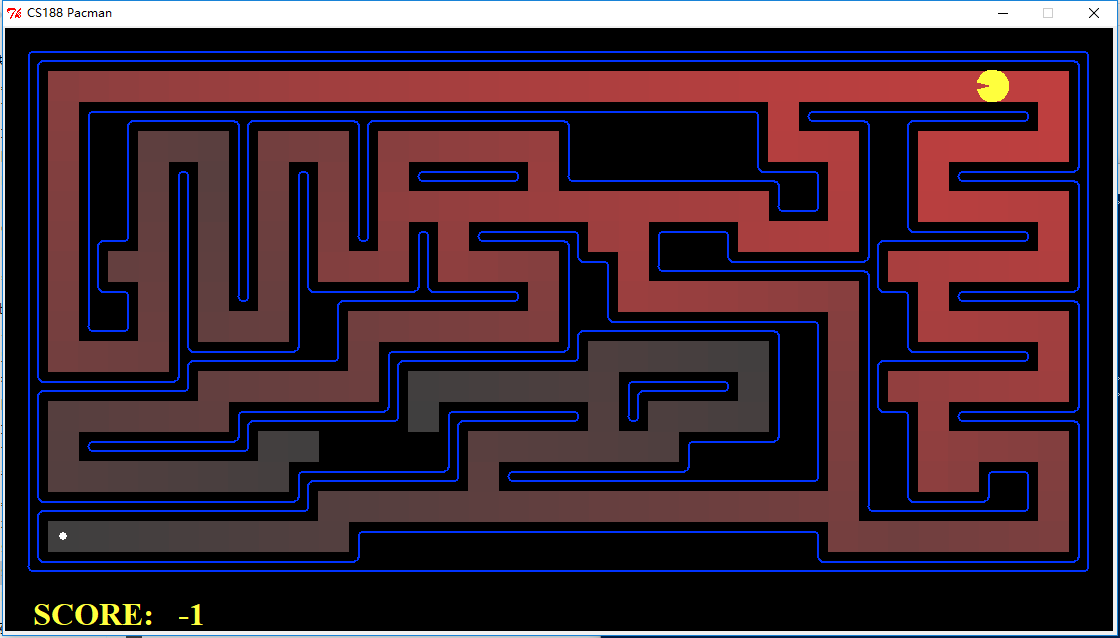
\includegraphics[width=15cm]{fig/Pacman}
\caption{Searching by BFS or DFS}
\end{figure}

\section{Codes}
\begin{lstlisting}
import sys
import time
import queue

if len(sys.argv) > 2:
	wallmark = '1'
	roadmark = '0'
	infile = "Maze1.txt"
else:
	wallmark = '%'
	roadmark = ' '
	infile = "Maze.txt"

# Initialization
maze = []
s, e = (0,0), (0,0)
best = ""
shortestLength = 0x3f3f3f3f

# Read in maze from file
with open(infile,"r") as file:
	for (i,line) in enumerate(file):
		if not line[-1] in [wallmark,'S','E',roadmark]:
			line = line[:-1]
		maze.append(line)
		j = line.find('S')
		if j != -1:
			s = (i,j)
		j = line.find('E')
		if j != -1:
			e = (i,j)

def validQ(x,y):
	"""
	Auxiliary function to test if (x,y) is a valid position to move to
	"""
	if y < 0 or y >= len(maze[0]) or x < 0 or x >= len(maze) or maze[x][y] in [wallmark,'*']:
		return False
	else:
		return True

def explore(x,y,d,visited,q):
	"""
	Auxiliary function for BFS

	(x,y): next position
	d: direction to the previous position, L, R, U, D
	visited: a bool array storing whether a position is visited
	"""
	if validQ(x,y) and visited[x][y] == 0:
		visited[x][y] = d
		q.append((x,y))

def BFS(x,y):
	"""
	Breath-First Search for the maze problem

	(x, y): the initial position
	"""
	global best, shortestLength
	# initialization
	q = [(x,y)]
	visited = []
	for i in range(len(maze)):
		visited.append([0]*len(maze[0]))
	visited[x][y] = -1
	# traversal
	while len(q) > 0:
		(x,y), q = q[0], q[1:]
		if (x,y) == e:
			break
		explore(x-1,y,'D',visited,q)
		explore(x+1,y,'U',visited,q)
		explore(x,y-1,'R',visited,q)
		explore(x,y+1,'L',visited,q)
	# generate the shortest path
	(x, y) = e
	shortestLength = 0
	while not visited[x][y] == -1:
		shortestLength += 1
		if visited[x][y] == 'D':
			x = x+1
		elif visited[x][y] == 'U':
			x = x-1
		elif visited[x][y] == 'L':
			y = y-1
		elif visited[x][y] == 'R':
			y = y+1
		maze[x] = maze[x][:y] + '*' + maze[x][y+1:]
	maze[s[0]] = maze[s[0]][:s[1]] + 'S' + maze[s[0]][s[1]+1:]
	for i in range(len(maze)):
		best += maze[i] + "\n"

def DFS(x,y,depth):
	"""
	Depth-First Search for the maze problem

	(x, y): the current position
	depth: current path length
	"""
	global best, shortestLength
	if not validQ(x,y):
		return
	if x == e[0] and y == e[1] and depth < shortestLength:
		shortestLength = depth
		best = ""
		maze[s[0]] = maze[s[0]][:s[1]] + 'S' + maze[s[0]][s[1]+1:]
		maze[e[0]] = maze[e[0]][:e[1]] + 'E' + maze[e[0]][e[1]+1:]
		for i in range(len(maze)):
			best += maze[i] + "\n"
		maze[s[0]] = maze[s[0]][:s[1]] + '*' + maze[s[0]][s[1]+1:]
		maze[e[0]] = maze[e[0]][:e[1]] + ' ' + maze[e[0]][e[1]+1:]
		return
	maze[x] = maze[x][:y] + '*' + maze[x][y+1:]
	DFS(x,y-1,depth+1)
	DFS(x+1,y,depth+1)
	DFS(x-1,y,depth+1)
	DFS(x,y+1,depth+1)
	maze[x] = maze[x][:y] + roadmark + maze[x][y+1:]

def heuristic(des,curr):
	"""
	Calculate the L1 distance
	"""
	return abs(des[0] - curr[0]) + abs(des[0] - curr[0])

def AStar(x,y):
	"""
	A* algorithm for the maze problem

	(x, y): the initial position
	"""
	global best, shortestLength
	# initialization
	q = queue.PriorityQueue()
	q.put((0,(x,y)))
	prev = {}
	prevCost = {}
	prev[s] = None
	prevCost[s] = 0
	# traversal
	while not q.empty():
		_, (x,y) = q.get()
		if (x,y) == e:
			break
		for pos in [(x-1,y),(x+1,y),(x,y-1),(x,y+1)]:
			newCost = prevCost[(x,y)] + 1
			if validQ(pos[0],pos[1]) and ((pos not in prev) or newCost < prevCost[pos]):
				prevCost[pos] = newCost
				priority = newCost + heuristic(e,pos)
				q.put((priority,pos))
				prev[pos] = (x,y)
	# generate shortest path
	p = e
	shortestLength = 0
	while prev[p] != None:
		shortestLength += 1
		x, y = p[0], p[1]
		maze[x] = maze[x][:y] + '*' + maze[x][y+1:]
		p = prev[p]
	maze[e[0]] = maze[e[0]][:e[1]] + 'E' + maze[e[0]][e[1]+1:]
	maze[s[0]] = maze[s[0]][:s[1]] + 'S' + maze[s[0]][s[1]+1:]
	for i in range(len(maze)):
		best += maze[i] + "\n"

# Initial state
start = time.time()
if sys.argv[1] == "DFS":
	DFS(s[0],s[1],0)
	name = "DFS"
elif sys.argv[1] == "BFS":
	BFS(s[0],s[1])
	name = "BFS"
elif sys.argv[1] == "A*":
	AStar(s[0],s[1])
	name = "A*"
end = time.time()

# Output
print(name,"Shortest length: ",shortestLength)
print("Running time: {:.4f}s".format(end-start))
print(best)
\end{lstlisting}


\section{Results}
In this experiment, I use three methods to find the shortest path of the maze, including BFS, DFS, and A$^\star$ algorithm.
The results are shown in Fig.~\ref{fig:res}.

The first line of each output gives the length of the shortest path of the problem, which are \textbf{all $68$} obtained by the three algorithms.

The second line shows the running time.
Surprisingly, \textbf{BFS runs the fastest, A$^\star$ ranks the second, and DFS is extremely slow}.
It may be caused by the relatively simple solution of the problem that A$^\star$ cannot show all its power.

The rest of the outputs show the maze and the shortest path which is marked out in \verb'*'.
We can see that all the three algorithms give correct solutions.

\begin{figure}[H]
\centering
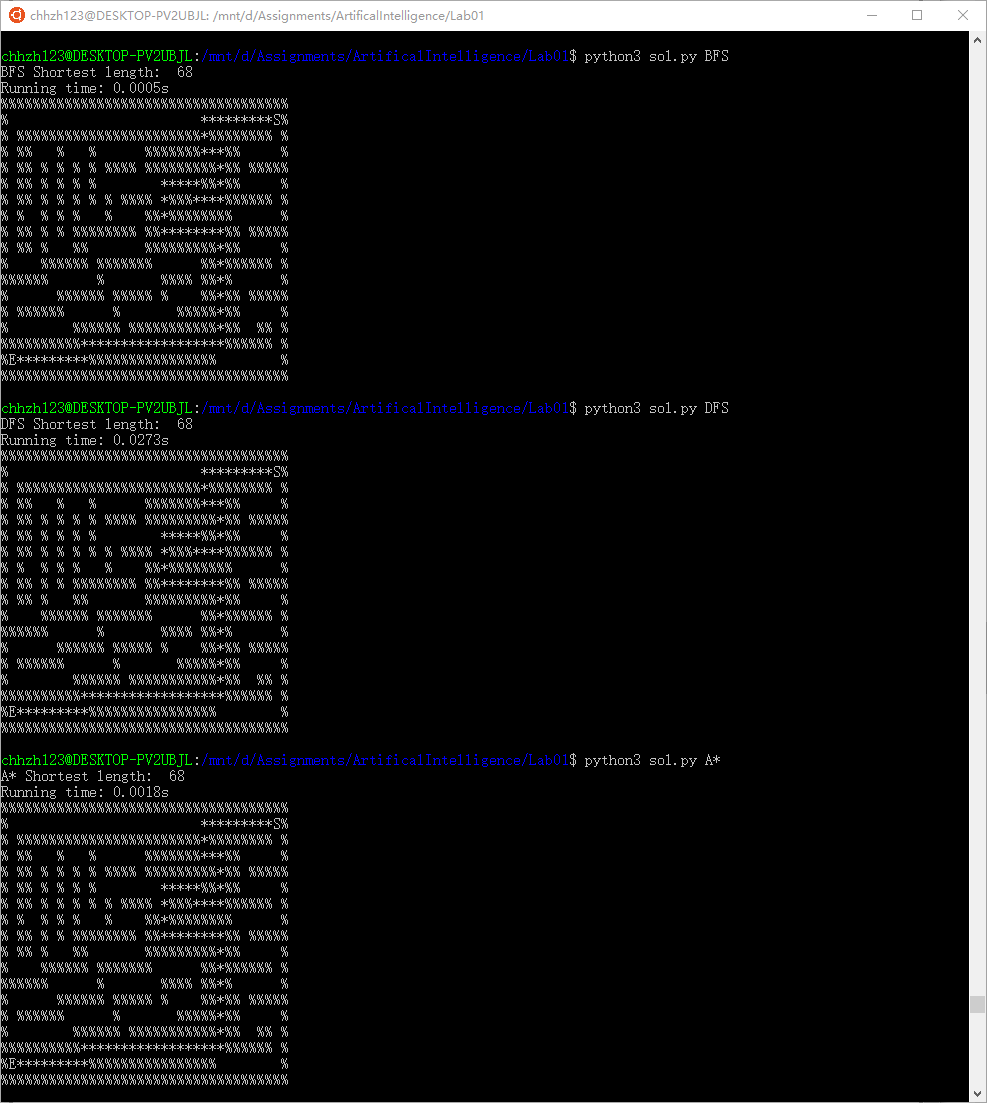
\includegraphics[width=\linewidth]{fig/results.png}
\caption{Experimental results of three search algorithms}
\label{fig:res}
\end{figure}


\begin{thebibliography}{99}
\bibitem{bib1} Red Blob Games, Introduction to the A$\star$ Algorithm, \url{https://www.redblobgames.com/pathfinding/a-star/introduction.html}
\end{thebibliography}

%\clearpage
%\bibliography{E:/Papers/LiuLab}
%\bibliographystyle{apalike}
\end{document}